\section{Randomized SVD}
Many matrices that appear in scientific contexts have a low rank structure which can 
be exploited. In recent years, the field of data science has also found low rank approximations
useful for their analysis. See the paper by \cite{udell-2019} for more on the topic.
The large size of data matrices can prohibit the direct calculation low rank structure, but
randomized methods can generate strong approximations. For a detailed analysis see the paper by
\cite{martinsson-2011} . Also Martinsson's website contains many slides and video lectures
on the topic. 
\subsection{The Singular Value Decomposition (SVD)}
The SVD is arguably the most important matrix decomposition in linear algebra.
Unlike the eigendecomposition, $LU$, and others, the SVD always exists and the
matrix need not be square. A SVD of $A\in\mathbb{R}^{m \times n}$ is

\begin{equation*}
A= U \Sigma V^{T}
\end{equation*}

Where $U\in \mathbb{R}^{(m \times m)}$ and $V \in \mathbb{R}^{(n \times n)}$ are
orthogonal and $\Sigma\in\mathbb{R}^{(m \times n)}$ is a diagonal matrix with
only non-negative entries.

\underline{Definition}

A matrix $U\in \mathbb{R}^{(m \times m)}$ is orthogonal if
\begin{enumerate}[1)]
\item The columns/rows are orthogonal
\item $U^{T}U = UU^{T} = I$
\item $U^{-1} = U^{T}$
\end{enumerate}

The diagonal entries of $\Sigma$ are denoted by $\sigma_1, \sigma_2, \ldots,
\sigma_p$ where $p=\min(m, n)$. We always order the columns of $U$, rows of
$V$, and diagonal of $\Sigma$ so that $\sigma_1 \geq \sigma_2 \geq \sigma_3 \geq
\ldots \geq \sigma_p \geq 0$

Having the SVD of a matrix is very useful. With an SVD, we can form the pseudo
inverse of $A$

\begin{equation*}
A^\dagger  = V \Sigma^\dagger U^T
\end{equation*}
where $\Sigma^\dagger$ is the transpose of $\Sigma$ and invert the non-zero
entries


\underline{Ex}
\begin{equation*}
  \Sigma =
  \begin{bmatrix}
    4 & 0 & 0 & 0 & 0 \\
    0 & 2 & 0 & 0 & 0 \\
    0 & 0 & 1 & 0 & 0 \\
    0 & 0 & 0 & 0 & 0 \\
  \end{bmatrix} \Rightarrow
  \Sigma^\dagger =
  \begin{bmatrix}
    1/4 & 0   & 0 & 0  \\
    0   & 1/2 & 0 & 0  \\
    0   & 0   & 1 & 0  \\
    0   & 0   & 0 & 0  \\
    0   & 0   & 0 & 0  \\
  \end{bmatrix}
\end{equation*}

%% Lecture 16
With the SVD, one can also find the best rank $r$ matrix that approximates $A$ with $r\leq \min(m,n)$

\begin{equation*}
\widetilde{A} = U \widetilde{\Sigma} V^T
\end{equation*}
where $\widetilde{\Sigma}$ is the matrix $\Sigma$ with only the first $r$ singular values

\begin{equation*}
    \Sigma =
    \begin{bmatrix}
        4 & 0 & 0 & 0 & 0 \\
        0 & 2 & 0 & 0 & 0 \\
        0 & 0 & 1 & 0 & 0 \\
        0 & 0 & 0 & 0 & 0 \\
    \end{bmatrix}
    , \quad r=2 \Rightarrow
    \widetilde{\Sigma} =
    \begin{bmatrix}
        4 & 0 & 0 & 0 & 0 \\
        0 & 2 & 0 & 0 & 0 \\
        0 & 0 & 0 & 0 & 0 \\
        0 & 0 & 0 & 0 & 0 \\
    \end{bmatrix}
\end{equation*}

This matrix $\widetilde{A}$ is the minimizer of
\begin{equation*}
    \big\{ \left\lVert A-B\right\rVert_2  | \text{rank}(B) = r \big\}
\end{equation*}

We can write our SVD using outer products as follows. Let $p=\min(m,n)$

\begin{equation*}
    A = U \Sigma V^T
\end{equation*}
\begin{equation*}
  A =
\begin{tikzpicture}[baseline=(current bounding box.center)]
    \matrix (m) [bmatrix,   nodes={outer sep=-\pgflinewidth,text depth=0.5ex,text height=2ex,text width=1.2em} ]{
    &&&\\
    &&&\\
    \Vec{u}_1&\Vec{u}_2&\ldots&\Vec{u}_m\\
    &&&\\
    &&&\\
    } ;
    \foreach \i in {1, 2, 4}
    \draw[->] (m-3-\i) -- (m-5-\i.south);
    \foreach \i in {1, 2, 4}
    \draw[->] (m-3-\i) -- (m-1-\i.north);
  \end{tikzpicture}
  \begin{bmatrix}
  \sigma_1 &&&\bigzero&\\
  & \sigma_2&&\\
  \bigzero& &\ddots&\\
  & &&\sigma_p\\
  \end{bmatrix}
\begin{tikzpicture}[baseline=(current bounding box.center)]
    \matrix (m) [bmatrix,   nodes={outer sep=-\pgflinewidth,text depth=0.5ex,text height=2ex,text width=1.2em} ]{
    &&\Vec{v}_1&&\\
    &&\Vec{v}_2&&\\
    &&\vdots&&\\
    &&\Vec{v}_n&&\\
    } ;
    \foreach \i in {1, 2, 4}
    \draw[->] (m-\i-3) -- (m-\i-1.west);
    \foreach \i in {1, 2, 4}
    \draw[->] (m-\i-3) -- (m-\i-5.east);
  \end{tikzpicture}
\end{equation*}
\begin{equation*}
    A = \sum_{i=1}^{p} \sigma_i \vec{u}_i \vec{v}^{\,T}_i
\end{equation*}

Unfortunately, computing the SVD directly requires $\bigO{mn^2}$ operations if $m \geq n$. For many practical problems, this is too expensive. Fortunately, many matrices in statistics, data sciences, PDEs, and more are \emph{numerically low rank}.

\underline{Definition}

Given a tolerence $\epsilon$, a matrix $A$ has numerical rank $k$ if there exists a rank $k$ matrix with
\begin{equation*}
    || A - \widetilde{A} || \leq \epsilon
\end{equation*}

$A$ is numerically low rank if $k$ is sufficiently small.

A very nice property to have is if the numerical rank of a matrix $A$ does \underline{\underline{not}} grow with the size of $A$, where the size of $A$ depends on how the problem is discretized.

To compute a low-rank approximation of $A\in \mathbb{R}^{m \times n}$, two computational tasks must be performed.

\begin{enumerate}[(A)]
    \item A low-dimensional subspace that captures the action of matrix $A$ must be formed.
    \begin{center}
\begin{tikzpicture}[
dot/.style={circle, inner sep=0pt, minimum size=3pt, fill=black}
]
    \begin{scope}
        \draw (0, 0) rectangle (5, 5);
        \node () at (2.5, 5.5) {$\mathbb{R}^{n}$};
        \node[dot, label=above left:$\Vec{x}$] (x) at (1.5, 4) {};
        \node[dot, label=below left:$\Vec{0}$] (x) at (2.5, 2.5) {};

        \node (rm) at (5, 2.5) {};

        \pgfmathsetseed{1}
        \foreach \i in {1, ..., 20}
           \pgfmathsetmacro{\x}{5*rnd}
           \pgfmathsetmacro{\y}{5*rnd}
            \node[dot] () at (\x, \y) {};
    \end{scope}

    \begin{scope}[xshift=7cm]
        \draw (0, 0) rectangle (5, 5);
        \node () at (2.5, 5.5) {$\mathbb{R}^{m}$};
        \node[dot, label=above right:$A\Vec{x}$] (x) at (1.2, 4) {};
        \node[dot, label=below left:$\Vec{0}$] (x) at (2.5, 2.5) {};
        \node (rn) at (0, 2.5) {};
        \begin{scope}
        \clip (0, 0) rectangle (5, 5);
        \pgfmathsetseed{7}
        \foreach \i in {1, ..., 20}
           \pgfmathsetmacro{\x}{(5*random())}
           \pgfmathsetmacro{\y}{5-(\x + 0.5*rand)}
            \node[dot] () at (\x, \y) {};
        \end{scope}
        \draw[red, dashed] (0, 5) -- (5, 0);

       \node[red, text width=3cm, anchor=south, yshift=.5cm] (text) at (5, 5) {low-dimentional subspace of the action/image of $A$} ;

       \draw[thick, red, ->] (text) to [bend right=10](2.2, 2.8);
    \end{scope}

    \draw[->](rm) to[bend left] node[above]{$A$} (rn);

\end{tikzpicture}
    \end{center}
    \item The matrix $A$ must be restricted to this subspace, and then a standard decomposition, such as an SVD is computed for the reduced matrix.
    \begin{equation*}
  A = \quad
\begin{tikzpicture}[baseline=0pt]
    \matrix (m) [bmatrix,   nodes={outer sep=-\pgflinewidth,text depth=0.5ex,text height=2ex,text width=1.2em}]{
    &&&&&&\\
    &&&&&&\\
    &&&&&&\\
    &&&&&&\\
    &&&&&&\\
    } ;
    \node[anchor=south east, xshift=-2em, yshift=-.3em] () at (m-3-1) {$m$};
    \node[anchor=south, yshift=2em] () at (m-1-4) {$n$};
  \end{tikzpicture}
\begin{tikzpicture}[baseline=1.8em]
    \matrix (m) [bmatrix,   nodes={outer sep=-\pgflinewidth,text depth=0.5ex,text height=2ex,} ]{
    \\
    \\
    \\
    \\
    \\
    \\
    \\
    } ;
    \node[anchor=south, yshift=1.75em, xshift=.3em] () at (m-1-1) {$\mathbb{R}^n$};
  \end{tikzpicture}
  =
\begin{tikzpicture}[baseline=0pt]
    \matrix (m) [bmatrix,   nodes={outer sep=-\pgflinewidth,text depth=0.5ex,text height=2ex,} ]{
    \\
    \\
    \\
    \\
    \\
    } ;
    \node[anchor=south, yshift=1.65em, xshift=.3em] () at (m-1-1) {$\mathbb{R}^m$};
  \end{tikzpicture}
\end{equation*}
\begin{equation*}
  B = \quad
\begin{tikzpicture}[baseline=0pt]
    \matrix (m) [bmatrix,   nodes={outer sep=-\pgflinewidth,text depth=0.5ex,text height=2ex,text width=1.2em}]{
    &&&&&&\\
    &&&&&&\\
    &&&&&&\\
    } ;
    \node[anchor=south east, xshift=-2em, yshift=-.3em] () at (m-2-1) {$k$};
    \node[anchor=south, yshift=2em] () at (m-1-4) {$n$};
  \end{tikzpicture}
\begin{tikzpicture}[baseline=3.3em]
    \matrix (m) [bmatrix,   nodes={outer sep=-\pgflinewidth,text depth=0.5ex,text height=2ex,} ]{
    \\
    \\
    \\
    \\
    \\
    \\
    \\
    } ;
    \node[anchor=south, yshift=1.75em, xshift=.3em] () at (m-1-1) {$\mathbb{R}^n$};
  \end{tikzpicture}
  =
\begin{tikzpicture}[baseline=0pt]
    \matrix (m) [bmatrix,   nodes={outer sep=-\pgflinewidth,text depth=0.5ex,text height=2ex,} ]{
    \\
    \\
    \\
    } ;
    \node[anchor=south, yshift=1.9em, xshift=.3em] () at (m-1-1) {$\mathbb{R}^k$};
  \end{tikzpicture}
\end{equation*}
\end{enumerate}

%% Lecture 17

More formally, task (A) is equivalent to the following:
\begin{displayquote}
    Compute an approximate basis for the range of $A$. This is equivalent to finding a matrix $Q\in\mathbb{R}^{m\times k}$ with orthonormal columns such that
    \begin{equation*}
        A \approx QQ^TA
    \end{equation*}
\end{displayquote}
This matrix $QQ^TA$ is what we called $\widetilde{A}$. We would also like $Q$ to have as few columns as possible. Ficen such a Q, we have

\begin{equation*}
    QQ^TA =  \widetilde{A}
\end{equation*}

Also,
\begin{equation*}
    A\vec{x} = Q\left(Q^TA\vec{x}\right) \in \text{Range}(Q)
\end{equation*}

\begin{equation*}
    \Rightarrow \text{Range}(A) \approx \text{Range}(Q)
\end{equation*}

\underline{Ex}

\begin{align*}
    A =
\begin{bmatrix}
    2 & 0 & 1 \\
    -1 & 3 & -2 \\
    2 & 0 & 1 \\
\end{bmatrix}
\end{align*}
The rank of $A$ is 2 and
\begin{equation*}
    \text{Range}(A) = \text{span}\left\{
\begin{bmatrix}
1\\-2\\1
\end{bmatrix},
\begin{bmatrix}
0\\1\\0
\end{bmatrix}
    \right\}
\end{equation*}

Let's make the following choice for $Q$

\begin{equation*}
    Q =
    \begin{bmatrix}
    1/\sqrt{3}&1/ \sqrt{6} \\
    1/\sqrt{3}&-2/\sqrt{6} \\
    1/\sqrt{3}&1/ \sqrt{6} \\
    \end{bmatrix}
\end{equation*}
\begin{align*}
    QQ^T &=
    \begin{bmatrix}
    1/\sqrt{3}&1/ \sqrt{6} \\
    1/\sqrt{3}&-2/\sqrt{6} \\
    1/\sqrt{3}&1/ \sqrt{6} \\
    \end{bmatrix}
    \begin{bmatrix}
    1/\sqrt{3} & 1/\sqrt{3} & 1/\sqrt{3} \\
    1/ \sqrt{6} &-2/\sqrt{6} &1/ \sqrt{6} \\
    \end{bmatrix}\\
    &=
    \begin{bmatrix}
        1/2 & 0 & 1/2 \\
        0 & 1 & 0 \\
        1/2 & 0 & 1/2 \\
    \end{bmatrix}
\end{align*}
\begin{align*}
    \Rightarrow QQ^TA &=
    \begin{bmatrix}
        1/2 & 0 & 1/2 \\
        0 & 1 & 0 \\
        1/2 & 0 & 1/2 \\
    \end{bmatrix}
\begin{bmatrix}
    2 & 0 & 1 \\
    -1 & 3 & -2 \\
    2 & 0 & 1 \\
\end{bmatrix}\\
&=
\begin{bmatrix}
    2 & 0 & 1 \\
    -1 & 3 & -2 \\
    2 & 0 & 1 \\
\end{bmatrix} = A
\end{align*}

That is, $A=QQ^TA$.

Given this matrix Q, we can perform task (B). For example, suppose we find a matrix $Q\in\mathbb{R}^{m\times k}$ with $A\approx QQ^TA$. Then we can do the following 3 steps
\begin{enumerate}[1)]
    \item Let $B=Q^TA$
    \item Compute the SVD of $B$ which is
    \begin{equation*}
        B = \widetilde{U}\Sigma V^T
    \end{equation*}
    \item Let $U=Q\widetilde{U}$
\end{enumerate}
Then,
\begin{align*}
U\Sigma V^T &= Q\widetilde{U} \Sigma V^T\\
&=QB\\
&=QQ^TA \approx A
\end{align*}
That is, $U\Sigma V^T$ is an approximate (truncated) SVD of $A$. The big question is

\begin{center}
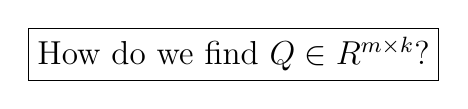
\begin{tikzpicture}
\node[font=\large, draw=black]() { How do we find $Q\in \mathbb{R}^{m \times k}$? };
\end{tikzpicture}
\end{center}

In this last example, I chose the optimal $3\times 2$ matrix $Q$ so that $||A-QQ^TA||$ is minimized. In fact, it was 0. In particular,


\begin{equation*}
A =
\begin{bmatrix}
    2 & 0 & 1 \\
    -1 & 3 & -2 \\
    2 & 0 & 1 \\
\end{bmatrix} =
\begin{bmatrix}
    -1/\sqrt{6} & -1/\sqrt{3}& -1/\sqrt{2} \\
    2/\sqrt{6} & -1/\sqrt{3} & 0 \\
    -1/\sqrt{6} & -1/\sqrt{3} & 1/\sqrt{2} \\
\end{bmatrix}
\begin{bmatrix}
    \sqrt{18} & 0 & 0 \\
    0& \sqrt{6} & 0 \\
    0& 0 & 0 \\
\end{bmatrix}
\begin{bmatrix}
     -1/\sqrt{3} & -1/\sqrt{2} & 1/\sqrt{6}\\
     1/\sqrt{3} & -1/\sqrt{2} & -1/\sqrt{6}\\
     -1/\sqrt{3} & 0           & -2/\sqrt{6}\\
\end{bmatrix}
\end{equation*}

Letting $Q$ be the left singular vectors of $A$ with a non-zero singular value, we have

\begin{equation*}
    Q =
    \begin{bmatrix}
    1/ \sqrt{6} & 1/\sqrt{3}\\
    -2/\sqrt{6} & 1/\sqrt{3}\\
    1/ \sqrt{6} & 1/\sqrt{3}\\
    \end{bmatrix}
\end{equation*}

%% Lecture 18

Last week, we looked for a matrix with orthonormal columns such that
\begin{equation*}
    A \approx QQ^TA \qquad \text{ with } A\in\mathbb{R}^{m\times n},\, Q \in \mathbb{R}^{m\times k}
\end{equation*}
The matrix $QQ^T$ is actually the matrix that does an orthogonal projection of any vector onto the space spanned by $Q$'s columns


\vspace{0.5cm}
\begin{center}
        \begin{tikzpicture}[
        point/.style={circle, fill=black, inner sep=0pt, minimum size=5pt}
        ]
        \draw[xslant=.2] (0, 0) rectangle (3, 3);
        \node[point, red] (x) at (2.5,3.5) {};
        \node[point] (zero) at (1,1.5) {};
        \node[fill=white, node distance=.1mm, below = of zero, xshift=-2mm] () {$\vec{0}$};
        \node[red, fill=white, right = .1em of x] () {$\vec{x}\in \mathbb{R}^m$};
        \begin{scope}[red, thick]
        \draw[dashed, thin] (zero) -- (zero)-|node[point, red](p){}(x)  -- (x);
        \draw[->] (zero) -- (x);
        \draw[->] (zero) -- (p);
        \node[] (QQT) at (2, -0.5) {$QQ^T\vec{x} \in \mathbb{R}^{m}$};
        \draw[->] (QQT) to[bend right =10] (p);
        \end{scope}
        \node[text width=3cm, anchor=west] (span) at (3.5, 1.5) {$\text{span}\{\vec{q_1}, \ldots, \vec{q}_k\} =\text{range}(Q)$};
        \draw[->] (span) to[bend right=10] (3, 2.5);
        \end{tikzpicture}\end{center}
\vspace{0.5cm}

Since we are computing $QQ^TA$, this is the orthogonal projection of the range of $A$ onto the space spanned by $Q$'s columns. Finally to see that $QQ^T$ is an orthogonal projection, recall that given any set of linearly independent vectors $\vec{q}_1, \ldots, \vec{q}_k \in \mathbb{R}^m$, but are not necessarily orthonormal, the matrix that performes an orthogonal projection onto, the space spanned by $\vec{q}_1, \ldots, \vec{q}_k$ is

\begin{equation*}
    P_Q = Q \left( Q^T Q \right)^{-1} Q^T
\end{equation*}

If $Q$ has orthogonal columns, then

\begin{equation*}
    Q^TQ =
    \begin{tikzpicture}[baseline=(current bounding box.center)]
        \matrix[
        matrix of math nodes,
        nodes={anchor=center},
        column 2/.style={nodes={fill=white}},
        nodes in empty cells,
        left delimiter={[},
        right delimiter={]},
        column sep = 1.5em
        ](V){
            & \vec{q}^{\,T}_1 &  \\
            & \vec{q}^{\,T}_2 &  \\[2em,between origins]
            &          &  \\[2em,between origins]
            & \vec{q}^{\,T}_k &  \\
        };
        \draw[dots, shorten <=1mm] (V-2-2) -- (V-4-2);
        \begin{scope}[on background layer]
        \draw[<->] (V-1-1.west) -- (V-1-3.east);
        \draw[<->] (V-2-1.west) -- (V-2-3.east);
        \draw[<->] (V-4-1.west) -- (V-4-3.east);
        \end{scope}
    \end{tikzpicture}
    \begin{tikzpicture}[baseline=(current bounding box.center)]
    \begin{scope}[
    every left delimiter/.style={xshift=1mm},
    every right delimiter/.style={xshift=-2mm}]
        \matrix[
        matrix of math nodes,
        %nodes={draw},
        row 2/.style={nodes={fill=white}},
        nodes in empty cells,
        left delimiter={[},
        right delimiter={]},
        row 2 column 4/.style={xshift=2pt},
        row sep = 2.1em
        ](U){
                      &            &[.5em]              &[.5em] \\
            \vec{q}_1 &  \vec{q}_2 &   & \vec{q}_k \\
                      &            &             & \\
        };
    \end{scope}
        \draw[dots] (U-2-2) -- (U-2-4);
        \begin{scope}[on background layer]
        \draw[<->] (U-1-1.north) -- (U-3-1.south);
        \draw[<->] (U-1-2.north) -- (U-3-2.south);
        \draw[<->] (U-1-4.north) -- (U-3-4.south);
        \end{scope}
    \end{tikzpicture}
\end{equation*}


\begin{align*}
    Q^TQ&=
    \begin{bmatrix}
        1 & 0 & \ldots & 0 \\
        0 & 1 & \ldots & 0 \\
        \vdots & \vdots & \ddots & \vdots \\
        0 & 0 & \ldots & 1 \\
    \end{bmatrix}
     = I \in \mathbb{R}^{k\times k} \\
     \Rightarrow P_Q &= QQ^T
\end{align*}

\underline{Aside about visualizing the SVD:}
\begin{center}
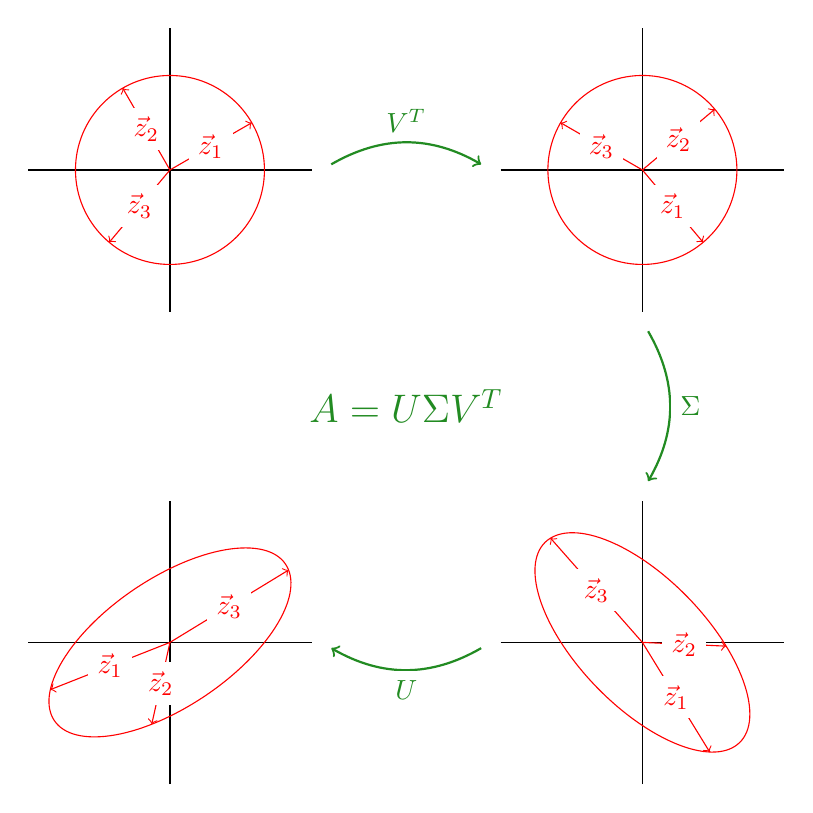
\begin{tikzpicture}[nodes={fill=white}, scale=1.2]
    \begin{scope}[xshift = 2.5cm, yshift=-2.5cm, ForestGreen, font=\Large]
        \node(){$A=U\Sigma V^T$};
    \end{scope}
    \begin{scope}
    \draw (-1.5, 0) -- (1.5, 0) node[right] (step1a){};
    \draw (0, -1.5) -- (0, 1.5);
    \begin{scope}[red]
    \draw (0, 0) circle (1);
    \draw[->] (0, 0) -- node[midway](){$\vec{z}_1$} (30:1);
    \draw[->] (0, 0) -- node[midway](){$\vec{z}_2$}(120:1);
    \draw[->] (0, 0) -- node[midway](){$\vec{z}_3$}(230:1);
    % \draw (0, 0) -- node[above](){$\vec{z}_1$} (30:1);
    % \draw (0, 0) -- node[left](){$\vec{z}_2$}(120:1);
    % \draw (0, 0) -- node[left](){$\vec{z}_3$}(230:1);
    \end{scope}
    \end{scope}
    \begin{scope}[xshift = 5cm]
        \draw (-1.5, 0) node[left](step1b){} -- (1.5, 0);
        \draw (0, -1.5) node[below](step2a){} -- (0, 1.5);
            \begin{scope}[rotate=-80, red]
                \draw (0, 0) circle (1);
    \draw[->] (0, 0) -- node[midway](){$\vec{z}_1$} (30:1);
    \draw[->] (0, 0) -- node[midway](){$\vec{z}_2$}(120:1);
    \draw[->] (0, 0) -- node[midway](){$\vec{z}_3$}(230:1);
            \end{scope}
    \end{scope}
    \begin{scope}[xshift = 5cm, yshift=-5cm]
        \draw (-1.5, 0) node[left](step3a){} -- (1.5, 0);
        \draw (0, -1.5) -- (0, 1.5) node[above](step2b){};
            \begin{scope}[red, rotate=-80, xslant=0.8]
                \draw (0, 0) circle (1);
    \draw[->] (0, 0) -- node[midway](){$\vec{z}_1$} (30:1);
    \draw[->] (0, 0) -- node[midway](){$\vec{z}_2$}(120:1);
    \draw[->] (0, 0) -- node[midway](){$\vec{z}_3$}(230:1);
            \end{scope}
    \end{scope}
    \begin{scope}[xshift = 0cm, yshift=-5cm]
        \draw (-1.5, 0) -- (1.5, 0) node[right](step3b){};
        \draw (0, -1.5) -- (0, 1.5);
            \begin{scope}[red, rotate=180, xslant=0.8]
                \draw (0, 0) circle (1);
    \draw[->] (0, 0) -- node[midway](){$\vec{z}_1$} (30:1);
    \draw[->] (0, 0) -- node[midway](){$\vec{z}_2$}(120:1);
    \draw[->] (0, 0) -- node[midway](){$\vec{z}_3$}(230:1);
            \end{scope}
    \end{scope}
    \draw[->,thick,  ForestGreen] (step1a) to[bend left] node[above](){$V^T$} (step1b);
    \draw[->, thick, ForestGreen] (step2a) to[bend left] node[right](){$\Sigma$} (step2b);
    \draw[->, thick, ForestGreen] (step3a) to[bend left] node[below](){$U$} (step3b);
\end{tikzpicture}
\end{center}


\underline{From previous example:}
\begin{equation*}
A =
\begin{bmatrix}
    2 & 0 & 1 \\
    -1 & 3 & -2 \\
    2 & 0 & 1 \\
\end{bmatrix} \qquad
Q =
\begin{bmatrix}
1/ \sqrt{6} & 1/\sqrt{3}\\
-2/\sqrt{6} & 1/\sqrt{3}\\
1/ \sqrt{6} & 1/\sqrt{3}\\
\end{bmatrix}
=
    \begin{tikzpicture}[baseline=(current bounding box.center)]
    \begin{scope}[
    every left delimiter/.style={xshift=1mm},
    every right delimiter/.style={xshift=-2mm}]
        \matrix[
        matrix of math nodes,
        %nodes={draw},
        row 2/.style={nodes={fill=white}},
        nodes in empty cells,
        left delimiter={[},
        right delimiter={]},
        row 2 column 4/.style={xshift=2pt},
        row sep = 1em
        ](U){
                      &             \\
            \vec{u}_1 &  \vec{u}_2  \\
                      &             \\
        };
    \end{scope}
        \begin{scope}[on background layer]
        \draw[<->] (U-1-1.north) -- (U-3-1.south);
        \draw[<->] (U-1-2.north) -- (U-3-2.south);
        \end{scope}
    \end{tikzpicture}
\end{equation*}


That is, $Q$'s columns are the left singular vectors of $A$ whose singular values are non-zero. Then


\begin{equation*}
    QQ^TA =
    \begin{tikzpicture}[baseline=(current bounding box.center)]
    \begin{scope}[
    every left delimiter/.style={xshift=1mm},
    every right delimiter/.style={xshift=-2mm}]
        \matrix[
        matrix of math nodes,
        %nodes={draw},
        row 2/.style={nodes={fill=white}},
        nodes in empty cells,
        left delimiter={[},
        right delimiter={]},
        row 2 column 4/.style={xshift=2pt},
        row sep = 1em
        ](U){
                      &             \\
            \vec{u}_1 &  \vec{u}_2  \\
                      &             \\
        };
    \end{scope}
        \begin{scope}[on background layer]
        \draw[<->] (U-1-1.north) -- (U-3-1.south);
        \draw[<->] (U-1-2.north) -- (U-3-2.south);
        \end{scope}
    \end{tikzpicture}
    \begin{tikzpicture}[baseline=(current bounding box.center)]
        \matrix[
        matrix of math nodes,
        nodes={anchor=center},
        column 2/.style={nodes={fill=white}},
        nodes in empty cells,
        left delimiter={[},
        right delimiter={]},
        column sep = 1.5em
        ](V){
            & \vec{u}^{\,T}_1 &  \\
            & \vec{u}^{\,T}_2 &  \\
        };
        \begin{scope}[on background layer]
        \draw[<->] (V-1-1.west) -- (V-1-3.east);
        \draw[<->] (V-2-1.west) -- (V-2-3.east);
        \end{scope}
    \end{tikzpicture}
    \begin{tikzpicture}[baseline=(current bounding box.center)]
    \begin{scope}[
    every left delimiter/.style={xshift=1mm},
    every right delimiter/.style={xshift=-2mm}]
        \matrix[
        matrix of math nodes,
        %nodes={draw},
        row 2/.style={nodes={fill=white}},
        nodes in empty cells,
        left delimiter={[},
        right delimiter={]},
        row 2 column 4/.style={xshift=2pt},
        row sep = 1em
        ](U){
                      &            & \\
            \vec{u}_1 &  \vec{u}_2 &\vec{u}_3  \\
                      &            & \\
        };
    \end{scope}
        \begin{scope}[on background layer]
        \draw[<->] (U-1-1.north) -- (U-3-1.south);
        \draw[<->] (U-1-2.north) -- (U-3-2.south);
        \draw[<->] (U-1-3.north) -- (U-3-3.south);
        \end{scope}
    \end{tikzpicture}
    \begin{tikzpicture}[baseline=(current bounding box.center)]
    \matrix[
    matrix of math nodes,
    nodes={anchor=center},
    nodes in empty cells,
    left delimiter={[},
    right delimiter={]}
    ](Sigma){
     \sigma_1 &         &   \\
              & \sigma_2&   \\
              &         & 0 \\
    };
\end{tikzpicture}
    \begin{tikzpicture}[baseline=(current bounding box.center)]
        \matrix[
        matrix of math nodes,
        nodes={anchor=center},
        column 2/.style={nodes={fill=white}},
        nodes in empty cells,
        left delimiter={[},
        right delimiter={]},
        column sep = 1.5em
        ](V){
            & \vec{v}^{\,T}_1 &  \\
            & \vec{v}^{\,T}_2 &  \\
            & \vec{v}^{\,T}_3 &  \\
        };
        \begin{scope}[on background layer]
        \draw[<->] (V-1-1.west) -- (V-1-3.east);
        \draw[<->] (V-2-1.west) -- (V-2-3.east);
        \draw[<->] (V-3-1.west) -- (V-3-3.east);
        \end{scope}
    \end{tikzpicture}
\end{equation*}

\begin{equation*}
    QQ^TA =
    \begin{tikzpicture}[baseline=(current bounding box.center)]
    \begin{scope}[
    every left delimiter/.style={xshift=1mm},
    every right delimiter/.style={xshift=-2mm}]
        \matrix[
        matrix of math nodes,
        %nodes={draw},
        row 2/.style={nodes={fill=white}},
        nodes in empty cells,
        left delimiter={[},
        right delimiter={]},
        row 2 column 4/.style={xshift=2pt},
        row sep = 1em
        ](U){
                      &             \\
            \vec{u}_1 &  \vec{u}_2  \\
                      &             \\
        };
    \end{scope}
        \begin{scope}[on background layer]
        \draw[<->] (U-1-1.north) -- (U-3-1.south);
        \draw[<->] (U-1-2.north) -- (U-3-2.south);
        \end{scope}
    \end{tikzpicture}
     \begin{bmatrix}
         1 & 0 & 0 \\
         0 & 1 & 0 \\
     \end{bmatrix}
     \Sigma V^T
\end{equation*}

\begin{equation*}
    QQ^TA =
    \begin{tikzpicture}[baseline=(current bounding box.center)]
    \begin{scope}[
    every left delimiter/.style={xshift=1mm},
    every right delimiter/.style={xshift=-2mm}]
        \matrix[
        matrix of math nodes,
        %nodes={draw},
        row 2/.style={nodes={fill=white}},
        nodes in empty cells,
        left delimiter={[},
        right delimiter={]},
        row 2 column 4/.style={xshift=2pt},
        row sep = 1em
        ](U){
                      &            & \\
            \vec{u}_1 &  \vec{u}_2 &\vec{0}  \\
                      &            & \\
        };
    \end{scope}
        \begin{scope}[on background layer]
        \draw[<->] (U-1-1.north) -- (U-3-1.south);
        \draw[<->] (U-1-2.north) -- (U-3-2.south);
        \draw[<->] (U-1-3.north) -- (U-3-3.south);
        \end{scope}
    \end{tikzpicture}
    \begin{tikzpicture}[baseline=(current bounding box.center)]
    \matrix[
    matrix of math nodes,
    nodes={anchor=center},
    nodes in empty cells,
    left delimiter={[},
    right delimiter={]}
    ](Sigma){
     \sigma_1 &         &   \\
              & \sigma_2&   \\
              &         & 0 \\
    };
\end{tikzpicture}
    \begin{tikzpicture}[baseline=(current bounding box.center)]
        \matrix[
        matrix of math nodes,
        nodes={anchor=center},
        column 2/.style={nodes={fill=white}},
        nodes in empty cells,
        left delimiter={[},
        right delimiter={]},
        column sep = 1.5em
        ](V){
            & \vec{v}^{\,T}_1 &  \\
            & \vec{v}^{\,T}_2 &  \\
            & \vec{v}^{\,T}_3 &  \\
        };
        \begin{scope}[on background layer]
        \draw[<->] (V-1-1.west) -- (V-1-3.east);
        \draw[<->] (V-2-1.west) -- (V-2-3.east);
        \draw[<->] (V-3-1.west) -- (V-3-3.east);
        \end{scope}
    \end{tikzpicture}
\end{equation*}
\begin{equation*}
    QQ^TA = \sigma_1 \vec{u}_1 \vec{v}^{\,T}_1 + \sigma_2 \vec{u}_2 \vec{v}^{\,T}_2 = A
\end{equation*}

%% Lecture 20

Of course, we can't use the SVD to construct $Q$ since the goal of computing $Q$ is to be able to compute the SVD and other matrix decompositions more efficiently. Instead we use \underline{randomized algorithms}. Again, our problem is the following:

\begin{displayquote}
Given a matrix $A \in \mathbb{R}^{m\times n}$ and a tolerance $\epsilon$, find a matrix $Q \in \mathbb{R}^{m\times k}$ with $k=k(\epsilon)$ and the columns of $Q$ being orthonormal such that
\begin{equation*}
    || A - QQ^TA || \leq \epsilon
\end{equation*}
where $||\cdot ||$ is the $l^2$-matrix norm
\end{displayquote}

If we find such a $Q$, the range of $Q$ is approximatly the $k$-dimensional (upto a tolerance $\epsilon$) range of $A$.

The SVD provides the best such $Q$. Letting $Q$ be the matrix with the first $k$ left singular vectors of $A$, we have $\text{rank}(Q)=k$ and
\begin{equation*}
    || A - QQ^TA || = \sigma_{k+1}
\end{equation*}

Therefore, given a tolerance $\epsilon$, if we could use the SVD to construct $Q$, we would choose $k$ such that $\sigma_{k+1} \leq \epsilon$ and $\sigma_k > \epsilon$.

In order to calculate $Q$ more effieciently, we start by introducing an oversampling parameter $p$. Assuming $A$ has rank $k$, our goal is now to find $Q$ with $k+p$ orthonormal columns such that
\begin{equation*}
    || A - QQ^TA || \approx \min_{\text{rank}(X)=k} || A- X||
\end{equation*}

As before, if $p=0$, the minimizer comes from the left singular vectors of $A$. However, by letting $p>0$, we have flexibility which will lead to more efficient methods.


Suppose $A \in \mathbb{R}^{m\times n}$ has rank $k$. We can draw a random vector $\vec{\omega} \in \mathbb{R}^n$ and compute $\vec{y} = A \vec{\omega} \in \text{range}(A)$.

We can repeat this $k$ times.

\begin{equation*}
    \vec{y}^{\,(i)} = A \vec{\omega}^{\,(i)} \qquad i = 1, 2, \ldots, k
\end{equation*}

Because we choose $\vec{\omega}^{\,(i)}$ randomly, the $\vec{y}^{\,(i)}$ are almost guaranteed to be linearly independent, and thus span range$(A)$. Then, to produce an orthonormal basis, we apply an algorithm such as Gram–Schmidt to generate $\vec{q}_1, \vec{q}_2, \ldots, \vec{q}_k$, and then

\begin{equation*}
    Q =
    \begin{tikzpicture}[baseline=(current bounding box.center)]
    \begin{scope}[
    every left delimiter/.style={xshift=1mm},
    every right delimiter/.style={xshift=-2mm}]
        \matrix[
        matrix of math nodes,
        %nodes={draw},
        row 2/.style={nodes={fill=white}},
        nodes in empty cells,
        left delimiter={[},
        right delimiter={]},
        row 2 column 4/.style={xshift=2pt},
        row sep = 1em
        ](U){
                      &            &[.5em]              &[.5em] \\
            \vec{q}_1 &  \vec{q}_2 &   & \vec{q}_k \\
                      &            &             & \\
        };
    \end{scope}
        \draw[dots] (U-2-2) -- (U-2-4);
        \begin{scope}[on background layer]
        \draw[<->] (U-1-1.north) -- (U-3-1.south);
        \draw[<->] (U-1-2.north) -- (U-3-2.south);
        \draw[<->] (U-1-4.north) -- (U-3-4.south);
        \end{scope}
    \end{tikzpicture}
\end{equation*}

is the matrix we need to construct. However, $A$ is in general not rank $k$, but has numerical rank $k$. That is
\begin{equation*}
    A = B + E
\end{equation*}
where $\text{rank}(B)=k$ and $||E||\leq\epsilon$. We wish to form a basis for the range of $B$. Since we are computing $A\vec{\omega}$, this vector is not in the range of $B$. Therefore, we choose more than $k$ vectors. In particular, we form the vectors
\begin{equation*}
    \vec{y}^{\,(i)} = A \vec{\omega}^{\,(i)} = B \vec{\omega}^{\,(i)} + E \vec{\omega}^{\,(i)} \qquad i = 1, 2, \ldots, k+p.
\end{equation*}
The perturbation $E \vec{\omega}^{\,(i)}$ shifts $\vec{y}^{\,(i)}$ from the range of $B$. Therefore, it is possible that $\vec{y}^{\,(1)}, \ldots, \vec{y}^{\,(k)}$ does not span the range of $B$. However the enriched space

\begin{equation*}
    \text{span} \left\{ \vec{y}^{\,(i)} \Big\vert i=1,\ldots, k+p\right\}
\end{equation*}
has a much better chance of spaning the range of $B$. Once we have chosen $p$, we have the beginnings of a basic algorithm to construct $Q\in \mathbb{R}^{m\times k}$ with
\begin{equation*}
    A \approx QQ^TA
\end{equation*}

Given a matrix $A \in \mathbb{R}^{m\times n}$, a target rank $k$, and an oversampling parameter $p$, the \emph{fixed-rank problem} computes a $m\times (k+p)$ matrix $Q$  whose columns are orthonormal and whose range approximates the range of $A$. The basic algorithm is as follows

\begin{enumerate}[1)]
    \item Draw a random $n \times (k+p)$ test matrix $\Omega$.
    \item Compute $Y = A \Omega \in \mathbb{R}^{m\times (k+p)}$.
    \item Construct a matrix $Q$ whose columns form an orthonormal basis for the range of $Y$.
\end{enumerate}

Note that we have not assumed that $Y$'s columns are linearly independent. Several issues that must be addressed are the following:
\begin{itemize}
    \item How large should we take $p$?
    \item What random matrix $\Omega$ should we pick?
    \item What if $k$ is not known in advanced?
    \item If $Y$ is ill-conditioned (which is likely), how do we stably orthonormalize its columns to generate $Q$?
    \item What computational cost is incurred?
\end{itemize}

%% Lecture 20


\underline{Theorem}

Let $A\in\mathbb{R}^{m\times n}$ and $k\geq2$ be a target rank and $p\geq2$ is an oversampling parameter such that $k+p\leq \min \{ m, n \}$

Then, if $\Omega\in\mathbb{R}^{n\times (k+p)}$ is a Gaussian test matrix used to generate $Y=A\Omega \in \mathbb{R}^{m \times (k+p)}$, and let $Q$ be the matrix with orthonormal vectors that span the range of $Y$. Then

\begin{equation*}
    \mathbb{E} || A - QQ^TA || \leq \left( 1 + \frac{4\sqrt{k+p}}{p-1}
    \sqrt{\min (m, n)}
    \right) \sigma_{k+1}
\end{equation*}
where $\mathbb{E}$ is the expected value and $\sigma_{k+1}$ is the $(k+1)$\textsuperscript{st} singular value of $A$.


\underline{Definition}

A Gaussian matrix is a matrix whose entries are all independently and identically distributed (iid) with distribution $\mathcal{N}(0, 1)$ (normal distribution with mean 0 and variance 1).

{\color{red}
In matlab you would do the following command to generate a Gaussian matrix

\begin{lstlisting}[language=Matlab]
Omega = randn(n, k+p)
\end{lstlisting}
}

A valid question to ask is what the variance of this distribution is (ie.\ $||A-QQ^TA||$). If it is large, then the estimate might not be very useful. However, one can show that if $\Omega$ is a Gaussian matrix in $\mathbb{R}^{n\times (k+p)}$
, then the probability that

\begin{equation*}
    ||AQQ^TA||\leq \left(1 + 9\sqrt{k+p}\sqrt{\min (m, n)}\right)\sigma_{k+1}
\end{equation*}
is at least $1-3p^{-p}$. Therefore, if $p=5$, we have about an $0.1\%$ chance that $||AQQ^TA||$ is larger than this bound. Therefore, we have addressed the issue about how to choose $p$.

\underline{Column Selection}

If we choose the columns of $\Omega$ to be one of the standard basis functions in $\mathbb{R}^n$

\begin{equation*}
    \vec{e}_i = (0, \ldots, 0, 1, 0, \ldots, 0)
\end{equation*}
then $\Omega$ will contain columns of $A$. By selecting columns, we have the following

\underline{Theorem}

Let $A\in\mathbb{R}^{m\times n}$ and $k\leq \min (m,n)$. Then, there exists a $k$-column submatrix $C\in\mathbb{R}^{k\times n}$ of $A$ for which

\begin{equation*}
    || A-CC^\dagger A || \leq \sqrt{1 + k(n-k)} || A-A_{(k)}||
\end{equation*}
where $A_{(k)}$ is the best rank $k$ approximation of $A$ (ie.\ it comes from the SVD) and $\dagger$ is the dagger operation for the pseudoinverse
\begin{equation*}
    C^\dagger = (C^TC)^{-1}C^T
\end{equation*}
Finding the optimal $C$ is an NP-hard problem. A more practical approach is to sample $A$'s columns randomly. But, we use the following heuristic. The columns of $A$ with the largest norm contribute ``the most" to the range of $A$. Therefore, we can create a distribution formed with the norms of $A$'s columns, and sample from this distribution.

This result is related to the \emph{Interpolative Decomposition} (ID). Given a matrix $A\in\mathbb{R}^{m \times n}$ of rank $k$, then there exists $k$ columns of $A$ that span all of the columns of $A$. That is, there exists an index set
\begin{equation*}
    J = \{j_1, \ldots, j_k \}
\end{equation*}
of positive integers less than $m$ with no repetition with
\begin{equation*}
    A = A_{(:, J) X}
\end{equation*}
with $X_{(:,J)} = I_k$. So far, this result is obvious since all columns of $A$ can be written as a linear combination of any $k$ columns of $A$ that span the range of $A$. What the ID guarantees that the entries of $X$ are bounded in absolute value by 2.

Let's form all possible IDs of the matrix
\begin{equation*}
    A =
    \begin{bmatrix}
        0 &  1 &  2 \\
        3 & -2 & -1 \\
        0 &  1 &  2 \\
    \end{bmatrix}
\end{equation*}
which has rank 2. We only have 3 choices for J.

Case 1: $J=\{1,2\}$

\begin{equation*}
    \begin{bmatrix}
        2\\
        -1\\
        2\\
    \end{bmatrix}
    =
    1
    \begin{bmatrix}
        0\\
        3\\
        0\\
    \end{bmatrix}
    +2
    \begin{bmatrix}
        1\\
        -2\\
        1\\
    \end{bmatrix}
    \Rightarrow
    A =
    \begin{bmatrix}
        0&1\\
        3&-2\\
        0&1\\
    \end{bmatrix}
    \begin{bmatrix}
        1&0&1\\
        0&1&2\\
    \end{bmatrix}
\end{equation*}
Since $|X_{ij}|\leq 2$, this is an ID.

Case 2: $J=\{2,3\}$
\begin{equation*}
    \begin{bmatrix}
        0\\
        3\\
        0\\
    \end{bmatrix}
    =
    -2
    \begin{bmatrix}
        1\\
        -2\\
        1\\
    \end{bmatrix}
    +1
    \begin{bmatrix}
        2\\
        -1\\
        2\\
    \end{bmatrix}
    \Rightarrow
    A =
    \begin{bmatrix}
        1&2\\
        -2&-1\\
        1&2\\
    \end{bmatrix}
    \begin{bmatrix}
        -2&1&0\\
        1&0&1\\
    \end{bmatrix}
\end{equation*}
This is an ID.

Case 3: $J=\{1,3\}$

\begin{equation*}
    \begin{bmatrix}
        1\\
        -2\\
        1\\
    \end{bmatrix}
    =
    \frac{-1}{2}
    \begin{bmatrix}
        0\\
        3\\
        0\\
    \end{bmatrix}
    +
    \frac{1}{2}
    \begin{bmatrix}
        2\\
        -1\\
        2\\
    \end{bmatrix}
    \Rightarrow
    A =
    \begin{bmatrix}
        0&2\\
        3&-1\\
        0&2\\
    \end{bmatrix}
    \begin{bmatrix}
        1&-1/2&0\\
        0&1/2&1\\
    \end{bmatrix}
\end{equation*}

%% Lecture 21

\underline{Gram-Schmidt}

One of the central tasks we need to do is form an orthonormal basis for the range (column space) of
the matrix $Y=A\Omega$, where $\Omega$ is some kind of random matrix. The standard way to form these
vectors is with \emph{Gram-Schmidt}(G-S).  G-S forms orthogonal vectors, $\vec{q}_1, \ldots, \vec{q}_{k+p}$, but they can be made orthonormal by normalizing
\begin{equation*}
    \vec{q}_i := \frac{\vec{q}_i}{||\vec{q}_i||} \qquad i=1, \ldots, k+p
\end{equation*}

To form the orthogonal vectors, suppose we start with $\vec{y}_1, \ldots, \vec{y}_k \in\mathbb{R}^m$. We then define $\vec{q}_1, \ldots, \vec{q}_k \in\mathbb{R}^m$ as follows:
\begin{align*}
    \vec{q}_1 &= \vec{y}_1 \\
    \vec{q}_2 &= \vec{y}_2 - \frac{\vec{q}^{\,T}_1\vec{y}_2}{\vec{q}_1^{\,T}\vec{q}_1}\vec{q}_1\\
    \vec{q}_3 &= \vec{y}_3 - \frac{\vec{q}^{\,T}_1\vec{y}_3}{\vec{q}_1^{\,T}\vec{q}_1}\vec{q}_1
    -
    \frac{\vec{q}^{\,T}_2\vec{y}_3}{\vec{q}_2^{\,T}\vec{q}_2}\vec{q}_2
    \\
    &\enspace\vdots \\
    \vec{q}_i &= \vec{y}_i - \sum_{j=1}^{i-1} \frac{\vec{q}^{\,T}_j\vec{y}_i}{\vec{q}_j^{\,T}\vec{q}_j}\vec{q}_j \qquad i=1, 2, \ldots, k.
\end{align*}

We can easily show that each of the $\{\vec{q}_1, \ldots, \vec{q}_{k}\}$ are in the span of $\{\vec{y}_1, \ldots, \vec{y}_{k}\}$

To see this, note that

\begin{align*}
    \vec{q}_1 &\in \text{span} \{ \vec{y}_1 \} \\
    \vec{q}_2 &\in \text{span} \{ \vec{q}_1, \vec{y}_2 \}
    \Rightarrow
    \vec{q}_2 \in \text{span} \{ \vec{y}_1, \vec{y}_2 \}
    \\
    &\vdots\\
    \vec{q}_i &= \text{span} \{ \vec{y}_1, \vec{y}_2, \ldots, \vec{y}_i \} \\
\end{align*}

The proof that $\vec{q}_1, \ldots, \vec{q}_{k}$ are orthogonal can be proved using mathematical induction.

One problem with G-S is that $\vec{q}^{\,T}_i\vec{q}_j$, $i \neq j$, is not quite 0 in finite precision because of rounding errors. This loss of orthogonality means $QQ^T$ is no longer an orthogonal projection, and this is a requirement for the approximation

\begin{equation*}
    A \approx QQ^TA
\end{equation*}

These vectors $\vec{q}_1, \ldots, \vec{q}_{k}$ can be computed in a different manner such that:

\begin{enumerate}[1)]
    \item The result is identical to the classical G-S in infinite precision.
    \item $\vec{q}^{\,T}_i\vec{q}_j$ willnot potentially be large because of round-off error.
\end{enumerate}
This method is know as modified G-S and it is numerically stable as opposed to classical G-S which is numerically unstable.

One nice feature of G-S is that it works even if $\vec{y}_1, \ldots, \vec{y}_{k}$ are linearly dependent. If this is the case, say $\vec{y}_i$ depends linearly on $\vec{y}_1, \ldots, \vec{y}_{i-1}$, then G-S will return $\vec{q}_i=\vec{0}$. We simply remove $\vec{y}_i$ from $Y$ and skip $\vec{q}_i$, and continue applying G-S.

\underline{The Fixed-Precision Problem}

So far, we have considered the problem of finding the best possible rank $k$ matrix whose range approximates the range of $A$.

This is called the \underline{fixed-rank problem} which involves finding $Q\in\mathbb{R}^{m\times k}$ with

\begin{equation*}
    ||A-QQ^TA||
\end{equation*}
as small as possible. However, we typically don't have a target rank, but instead have a target tolerance. This results in the \underline{fixed precision problem}:

\begin{displayquote}
    Given a tolerance $\epsilon > 0$, find a matrix $Q\in\mathbb{R}^{m\times l}$ with orthonormal columns and $l$ as small as possible such that
    \begin{equation*}
        ||QQ^TA-A||\leq \epsilon
    \end{equation*}
\end{displayquote}

The size of $l$ must be at least as large as the $\epsilon$-rank of $A$, but we want to keep $l$ as close to $k$ as possible. The idea is to generate $Q$ one column at a time, and check $||QQ^TA-A||<\epsilon$ at each iteration. 

%% Lecture 22


The size $l$ should only be slightly larger than the $\epsilon$-rank of $A$ which is $k$. We could simply construct columns of $Q$ one at a time, and check if $|| QQ^TA-A|| \leq \epsilon$ at each iterations. However, this is too expensive.

Instead of computing the matrix norm at each iteration, we might expect that applying $QQ^TA-A$ to a random vector can tell us something about its norm. We will use the following result.

\underline{Theorem}

Let $\left\{ \vec{\omega}^{\,(i)}, i=1, \ldots, r\right\}$ be $r$ standard Gaussian vectors. Then ,
\begin{equation*}
    || QQ^TA-A|| \leq 10 \sqrt{\frac{2}{\pi}}\max_{i=1, \ldots, r} ||(QQ^T - I)A\vec{\omega}^{\,(i)}||
\end{equation*}
with probability at least $1-10^{-r}$

Therefore, if we let $r=4$, then by computing 4 vector norms, we have a bound on $||QQ^TA-A||$ with probability $1-10^{-4} = 99.99\%$.

This result allows us to incrimentally construct $Q$ so that $QQ^TA\approx A$. We start with $Q^{(0)}$ being the empty matrix


\begin{algorithm}
    % \caption{Construct $Q$ so that $QQ^TA\approx A$.}
    \begin{algorithmic}
    \FOR{$i=1, 2, \ldots$}
      \STATE Let $\vec{\omega}^{\,(i)} \in \mathbb{R}^n$ be a Gaussian random vector.
      \STATE Let $\vec{y}^{\,(i)} = A\vec{\omega}^{\,(i)}$ \qquad {\color{red} \% $\vec{y}^{\,(i)}$ is in the range of $A$}
      \STATE Compute $\widetilde{\vec{q}}^{\,(i)} = \left( I - Q^{(i-1)}Q^{(i-1)T} \right)\vec{y}^{\,(i)}$
      {\color{red}
      \STATE \quad \% orthogonal projection of $\vec{y}^{\,(i)}$ onto the
      \STATE \quad \% column space of $Q^{(i-1)}$
      }
      \STATE Normalize $\vec{q}^{\,(i)} = \widetilde{\vec{q}}^{\,(i)} / ||\widetilde{\vec{q}}^{\,(i)}||$
      \STATE Update $Q^{(i)} = Q^{(i-1)} \vec{q}^{\,(i)}$
    \ENDFOR
      \end{algorithmic}
  \end{algorithm}
We break the loop when we believe that $||Q^{(l)}Q^{(l)T}A-A|| \leq \epsilon$, but how do we choose $l$? Using the last Theorem, we can show that $||(QQ^T - I)A\vec{\omega}^{\,(i)}||$ can be used to estimate the matrix norm, but this is exactly $||\widetilde{\vec{q}}^{\,(i)}||$. Therefore, we stop when we observe $r$ consecutive vectors $||\widetilde{\vec{q}}^{\,(i)}||$ with norms less than $\epsilon/(10\sqrt{2/\pi})$


